\chapter{Pythonin asennus ja tekstin tulostaminen}

\section{Yleistietoa Pythonista}

Python on yleiskäyttöinen ohjelmointikieli, johon tämä teos keskittyy. Aloittelijoille kieltä suositellaan sen yksinkertaisuuden ja käyttäjäystävällisyyden vuoksi; ammattikäytössä Pythoniin törmää usein tieteellisessä tutkimuksessa, mutta sillä on mahdollista myös esimerkiksi palvelinohjelmointi ja peliohjelmointi. Ominaisuuksiltaan Python on lähellä 2010-luvun muita käytetyimpiä ohjelmointikieliä (mm. Java, C, C++, JavaScript), minkä vuoksi sen parissa oppii varmasti hyödyllisiä taitoja, jotka helpottavat muihin kieliin siirtymistä.

Ensimmäisen version Pythonista julkaisi Guido van Rossum vuonna 1991, ja nykyisin sen kehityksestä vastaa Python Software Foundation (\url{https://www.python.org/}). Säätiön sivuilta löytyy kattava englanninkielinen Python-opas (\url{https://docs.python.org/3/tutorial/}) sekä Pythonin \gls{dokumentaatio} (\url{https://docs.python.org/3/}) eli yksityiskohtainen kuvaus kaikista Pythonin sisäänrakennetuista ominaisuuksista (ymmärtäminen vaatii perustiedot Pythonista).

\section{Tästä kirjasta}

Tämä hyvin keskeneräinen oppikirja on tarkoitettu lukion kurssimateriaaliksi ohjelmointia vähän tai ei lainkaan harrastaneille. Pyrin Pythonin alkeiden opettamisen lisäksi yleissivistämään lukijaa tietojenkäsittelytieteen maailmasta; tätä varten käytän muutamia käsitteitä, joita ei erikseen tarvitse opetella, jos se ei mielekkäältä tunnu. Sanasto kirjan lopussa toivottavasti auttaa, jos jonkin sanan merkitys on epäselvä.

Oppimisen tukena kannattaa käyttää (tai on pakko käyttää, jos kirja valmistuu hitaammin kuin opiskelet) tässä luvussa listattuja muita Python-oppaita.

Kirjan tehtävät ovat pääasiallisesti peräisin Helsingin yliopiston Python-kurssimateriaalista (\url{https://www.cs.helsinki.fi/group/linkki/materiaali/python-perusteet/materiaali.html}) sekä Ohjelmointiputkan Python-oppaasta (\url{https://www.ohjelmointiputka.net/oppaat/opas.php?tunnus=python_01}). Tarkemmat lähdetiedot on merkitty tehtäviin.

\section{Python 2 vai Python 3?}

Python-ohjelmointia aloittava voi törmätä yllättävään ongelmaan: edes oppaan ensimmäinen, yhden rivin esimerkkikoodipätkä ei toimi. Kyse on siitä, että Pythonista on yhä käytössä useita eri versioita: vanhempi Python 2 ja uudempi Python 3.

Kirjoitushetkellä Python 3:n julkaisuhetkestä alkaa olla jo kymmenisen vuotta, mikä on valtavan pitkä aika tietotekniikan maailmassa. Erinäisistä syistä (kuten siitä, että useat kirjastot toimivat yhä vain Python 2:lla) Python-ohjelmoijat ovat kuitenkin vaihtaneet uudempaan versioon melko hitaalla tahdilla, eikä ole epätodennäköistä, että uudetkin Python-oppaat opettavat vanhaa Python 2:ta.

Totuus on kuitenkin se, että aloittelijan ei ole mitään syytä olla käyttämättä Python 3:a. Se on ainut Python-versio, johon enää tulee uusia ominaisuuksia ja bugikorjauksia -- Python 2:n aktiivinen kehitys loppui jo viisi vuotta sitten. Suomenkielistä ohjelmoijaa ilahduttaa lisäksi se, että ääkköset toimivat Python 3:ssa ilman sen erityisempää säätämistä. Siispä tämä kirja opettaa asiat Python 3 -tavalla; jos näet virheilmoituksia, kokeile muuttaa koodistasi tällaiset rivit

\begin{python}
print "tekstin tulostaminen"
\end{python}

tällaisiksi

\begin{python}
print("tekstin tulostaminen")
\end{python}

Toinen usein esiin tuleva ero on, että \code{raw\_input()}-funktion nimi on Python 3:ssa pelkkä \code{input()}.

Jos tietokoneessasi on jo asennettuna Python, varmista, että kyseessä on uudempi versio. Useissa Linux-pohjaisissa käyttöjärjestelmissä on molemmat; jos \code{python}-komento avaa Python 2:n, kokeile komentoa \code{python3} (sama pätee myös kaikkiin Python-työkaluihin).

\section{Ympäristön asentaminen}

Pythonin voi ladata osoitteesta \url{https://www.python.org/downloads/} (muista valita Python 3!). Windowsilla ja Macilla mukana tulee IDLE-niminen ohjelma, jonka avulla Python-koodia voi kirjoittaa ja suorittaa kätevästi.

Linux-pohjaisilla käyttöjärjestelmillä jokin versio Pythonista on hyvin todennäköisesti jo asennettu. Jos näin ei ole (tai koneella on Python 2), Python tulee asentaa omaa pakettienhallintaohjelmaa käyttäen; lisäksi IDLE-ohjelma todennäköisesti puuttuu. Esimerkiksi Ubuntussa ne asennetaan syöttämällä konsoliin seuraavat komennot:

\begin{bash}
$ sudo apt install python3
$ sudo apt install idle3
\end{bash}

Lyhyt huomio notaatiosta: merkkiä $\$$ komennon alussa ei syötetä konsoliin, vaan sitä käytetään tavanomaisesti erottamaan ohjeissa komennot ja se, mitä komennot tulostavat konsoliin. Asentaakseen Pythonin käyttäjä siis kirjoittaa \code{sudo apt install python3}

Pythonin asennukseen liittyviin ongelmiin löytyy todennäköisesti vastaus Googlesta.

\section{Lyhyt IDLE-esittely}

Kun \gls{IDLE}-ohjelman avaa, näkyviin ilmestyy tällainen näkymä.

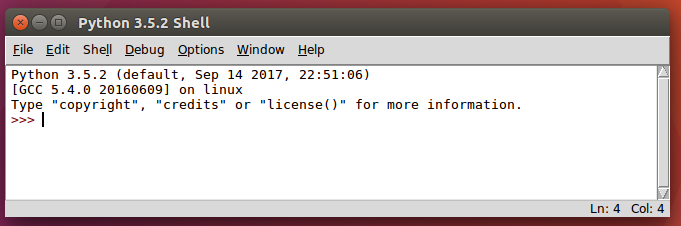
\includegraphics[width=10cm]{IDLE_shell}

Kyseessä on Python-\gls{komentotulkki} -- ohjelma, joka suorittaa välittömästi siihen syötetyn Python-koodin. Jos niin haluaa, kaikki Python-ohjelmansa voi syöttää rivi riviltä komentotulkkiin, mutta kätevämpää on pitää ne erillisissä tiedostoissa. Valitsemalla \code{File -> New File} avautuu IDLE:n tiedostoeditori.

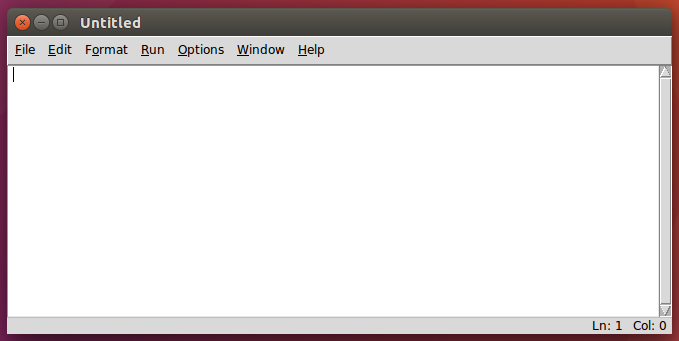
\includegraphics[width=10cm]{IDLE_newfile}

Kun Python-ohjelmansa on kirjoittanut IDLE:n koodieditorilla, sen voi suorittaa painamalla \code{F5}.

\section{Pythonin käyttäminen komentoriviltä}

Aloittelija pärjää hyvin graafisilla työkaluilla, mutta halutessaan kaiken tässä kirjassa esitetyn voi tehdä Pythonin komentorivityökaluilla. Konsolin saa auki Windowsilla painamalla \code{Windows + R} ja kirjoittamalla \code{cmd}, Unix-pohjaisilla käyttöjärjestelmillä (mm. OSX ja eri Linuxit) yleensä painamalla \code{CTRL + ALT + T}.

Alla on muistin virkistämiseksi taulukoituna peruskomennot, joiden avulla esimerkkien suorittamisen pitäisi onnistua.

\begin{tabularx}{\textwidth}{ |X|X|X| }
\hline
\textbf{Windows-komento} & \textbf{Unix-komento} & \textbf{Selitys} \\ \hline
\code{cd \textit{kansio}} & \code{cd \textit{kansio}} & Siirtyy annettuun kansioon \\
\code{dir} & \code{ls} & Tulostaa nykyisen kansion sisältämät tiedostot \\
\code{help \textit{komento}} & \code{man \textit{komento}} & Näyttää lisätietoja annetusta komennosta \\
\code{python} & \code{python} tai \code{python3} & Avaa interaktiivisen Python-komentotulkin \\
\code{python \textit{tiedosto}} & \code{python \textit{tiedosto}} tai \code{python3 \textit{tiedosto}} & Suorittaa annetun Python-tiedoston \\
\hline
\end{tabularx}

Seuraa lyhyt esimerkkisessio, jonka aikana Unix-pohjaista käyttöjärjestelmää käyttävä henkilö siirtyy \code{python}-kansioon tiedostojärjestelmässään, listaa sen sisältämät tiedostot ja suorittaa \code{kiva\_ohjelma.py}-nimisen tiedoston, joka tulostaa ruudulle viestin \code{Se toimii!}.

\begin{bash}
$ cd python
$ ls
kiva_ohjelma.py
toinen_ohjelma.py
oppikirja.pdf
$ python kiva_ohjelma.py
Se toimii!
\end{bash}

Kuten edellisessä esimerkissä, $\$$ komentojen alussa ei ole osa komentoa vaan erottaa komennot ja niiden tulostaman tekstin.

Aihetta voisi käsitellä enemmänkin, mutta tässä vaiheessa Python-opintoja se ei ole kovin mielekästä. Konsolin käytöstä innostunut tai ongelmia kohdannut lukija voi turvautua Googleen.

\section{Ensimmäinen ohjelma}

Ensimmäisistä ohjelmista klassisin on yksinkertainen sovellus, joka tulostaa ruudulle tekstin \code{Hei maailma!}

Alla on esitetty Hei maailma -ohjelman Python-toteutus. Kirjoita se IDLE:n avulla tiedostoon ja suorita painamalla \code{F5}. 

\begin{example}{Hei maailma!}
print("Hei maailma!")
\end{example}

Jos onnistuit, teksti \code{Hei maailma!} tulostui IDLE:n komentotulkkiin sinisellä värillä.

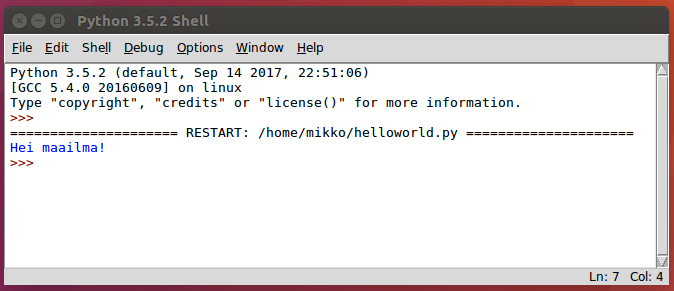
\includegraphics[width=10cm]{IDLE_helloworld}

Vastedes sitä, mitä Python-koodi tulostaa ruudulle, merkitään tässä kirjassa näin.

\begin{output}
Hei maailma!
\end{output}

Jos saat virheilmoituksen, palaa ensin tämän kirjan selostukseen Python 2:n ja Python 3:n eroista ja varmista, että sinulla on asennettuna Python 3. Vika voi olla myös koodissa itsessään -- tarkista, että kopioit esimerkkiohjelman merkilleen oikein. Aloitteleva ohjelmoija huomaa nopeasti, että toisin kuin ihminen, tietokone ei yritä arvailla, mitä käyttäjä on voinut tarkoittaa: jos vaikkapa viimeisen sulun unohtaa, on seurauksena virhe, vaikka onkin ilmiselvää, mitä ohjelmoija on halunnut tehdä.

Kun ohjelman saa toimimaan, koittaa aika leikkiä. Muuta tulostettavaa tekstiä muuttamalla lainausmerkkien sisältöä tai kokeile laittaa useampi tulostus peräkkäin kirjoittamalla useita rivejä, joissa on jokaisessa \code{print()} ja sulkujen sisällä haluttu teksti merkkijonojen välissä. Tehtävissä on lisäehdotuksia.

Vaikka luvun ainut esimerkki onkin yksinkertainen, se täyttää Python-ohjelman määritelmän. Python-ohjelma koostuu (yksinkertaistetusti) \glslink{lause}{lauseista}. Ohjelmassamme on yksi ainoa lause: \code{print("Hei maailma!")}. Se on tarkemmin sanottuna \textit{funktiokutsu}, jossa \glslink{funktio}{funktiolle} \code{print} annetaan \textit{argumenttina} teksti \code{Hei maailma!}, joka on tarkennettuna \gls{merkkijono}. Myöhemmin tutustutaan toisiin funktioihin, joilla voimme tehdä muutakin kuin vain tulostaa tekstiä.

Funktioihin ja merkkijonoihin palataan tulevissa luvuissa.

\section{Useiden rivien tulostaminen}

Edellisen osion lyhyt esimerkkiohjelma tulostaa Python-konsoliin yhden ainoan rivin tekstiä. Jos rivejä haluaa useampia, voi toimia monella tavalla; helpointa on yksinkertaisesti kirjoittaa monta \code{print}-lausetta, joista jokainen tulostaa oman rivinsä. Tässä havainnollistava esimerkki.

\begin{python}
print("Ensimmäinen rivi...")
print("... ja toinen.")
\end{python}

Esimerkki tulostaa näytölle seuraavan tekstin:

\begin{output}
Ensimmäinen rivi...
... ja toinen.
\end{output}

Muitakin tapoja on. Kenoviivaa (\code{\textbackslash}) voidaan käyttää \glslink{koodinvaihtomerkki}{koodinvaihtomerkkinä}, jolloin sen avulla voidaan kirjoittaa rivinvaihtomerkki (\code{\textbackslash n}). Rivinvaihtomerkin kohdatessaan Python jatkaa tekstiä uudelta riviltä, joten seuraavalla esimerkillä on tismalleen sama ulostulo.

\begin{python}
print("Ensimmäinen rivi...\n... ja toinen.")
\end{python}

Näin on tehtävä, koska Python ei salli merkkijonon jatkuvan seuraavalle riville. Tämä rajoitus kuitenkin poistuu, jos yhden lainausmerkin sijaan merkkijonon alussa ja lopussa käytetään kolmea.

\begin{python}
print("""Ensimmäinen rivi...
... ja toinen.""")
\end{python}

\section{Kommentointi}

Kommentit ovat hyödyllinen työkalu, jonka avulla koodiin voi jättää pieniä merkintöjä. Seuraava esimerkki havainnollistaa kommenttien eri käyttötarkoituksia; kommentti alkaa \code{\#}-merkistä ja jatkuu rivin loppuun saakka. Python-tulkki jättää huomiotta kaiken kommentissa olevan, joten kommenttien sisältö ei vaikuta mitenkään ohjelman toimintaan, mutta joitakin käyttötarkoituksia niillä siitä huolimatta on.

\begin{example}{Kommennointi}
# Koodannut Olli Ohjelmoija 4.10.2017
# Erkki Esimerkki korjasi bugin 6.10.2017

# Tulostaa tekstin "kissa"
print("kissa")

# print("koira")
\end{example}

Ensinnäkin kommenteilla voi jättää koodiin tietoja siitä, minkälaisia muutoksia eri henkilöt ovat siihen tehneet. Nykyisin tämä hoidetaan yleensä erillisellä \glslink{versiohallintaohjelma}{versiohallintaohjelmalla}, mutta aloittelijoiden ryhmätyössä voi olla kätevintä käyttää koodin alkuun sijoitettavia kommentteja.

Tämän lisäksi kommenteilla voidaan selittää, mitä hankalat tai muuten epäselvät pätkät koodia tekevät. Aloittelija voi toki jättää itselleen esimerkin kaltaisia kommentteja, jotka edistyneemmälle ohjelmoijalle ovat täysin turhia, mutta yleensä kannattaa miettiä kriittisesti kommenttien tarpeellisuutta – tarpeettomat kommentit voivat lisätä koodin lukemisen hankaluutta. Hyvä nyrkkisääntö on, että kommenttien pitäisi kertoa, \textit{miksi} sen kirjoittanut ohjelmoija päätyi juuri valitsemaansa ratkaisuun; koodi voi puhua omasta puolestaan.

Esimerkin kolmas kommentti näyttää, kuinka tietyn koodirivin voi nopeasti ottaa pois käytöstä muuttamalla sen kommentiksi. Todettakoon kuitenkin, että on huonoa tyyliä jättää koodiin sadoittain pois kommentoituja rivejä – kuten turhat ja itsestäänselvät kommentit, nekin saavat koodia lukevan henkilön kiinnittämään huomionsa itseensä. Jos kommentoituja koodirivejä projektiinsa kuitenkin jättää, on hyvätapaista kirjoittaa selventävä kommentti, joka selittää, miksi rivit on otettu pois käytöstä.

\section{Tehtäviä}

\begin{enumerate}[\thesection .1]
\item Muuta esimerkkiohjelma 1.1 tulostamaan oma nimesi.
\item Muokkaa esimerkkiohjelmaa 1.1. Kokeile, mitä käy, jos...
	\begin{enumerate}
	\item ... viimeisen sulun poistaa
	\item ... viimeisen lainausmerkin poistaa
	\item ... lainausmerkkien sisällä ei ole mitään
	\item ... \code{print}-funktion kirjoittaa väärin (vaikkapa \code{pirnt})
	\end{enumerate}
\item Kokeile eri tapoja tulostaa useita rivejä tekstiä. Tee ainakin kaksi ohjelmaa, jotka tulostavat

\begin{output}
Hei maailma!
Englanniksi se on Hello, World!
\end{output}

\item Mitä hyötyä kommenteista on, jos ne voisi poistaa, eikä ohjelma muuttuisi mitenkään?

\end{enumerate}
